\documentclass[11pt,twoside]{article}

% ============================================================
% Estilo de composición, aproximación a DADOS
% ============================================================

% --- Idiomas ---
\usepackage[utf8]{inputenc}
\usepackage[T1]{fontenc}
\usepackage[portuguese,english,spanish]{babel}

% --- Tipografía ---
\usepackage{newtxtext}
\usepackage{newtxmath}
\usepackage{microtype}

% --- Geometría ---
\usepackage[a4paper,margin=2.6cm]{geometry}

% --- Párrafos ---
\setlength{\parindent}{0pt}
\setlength{\parskip}{7pt}
\raggedbottom

% --- Gráficos y tablas ---
\usepackage{graphicx}
\graphicspath{{tablasyfig/}}
\usepackage{booktabs}
\usepackage{longtable}
\usepackage{tabularx}
\usepackage{array}
\usepackage{ragged2e}
\usepackage{float}
\usepackage{placeins}
\usepackage{caption}
\usepackage{subcaption}
\newcolumntype{P}[1]{>{\RaggedRight\arraybackslash}p{#1}}

% --- Listas (uso restringido, evitar en intro y discusión) ---
\usepackage{enumitem}
\setlist{leftmargin=*}

% --- Números (coma decimal) ---
\usepackage[output-decimal-marker={,}]{siunitx}
\sisetup{output-decimal-marker={,}, group-separator={.}, group-minimum-digits=4}

% --- TikZ (solo si se usa el diagrama de flujo) ---
\usepackage{tikz}
\usetikzlibrary{arrows.meta,positioning,calc,fit,backgrounds}

% --- Hipervínculos ---
\usepackage[hidelinks]{hyperref}

% --- Citas ---
\usepackage[round,authoryear]{natbib}

% --- Encabezados y pie (estilo DADOS aproximado) ---
\usepackage{lastpage}
\usepackage{fancyhdr}
\pagestyle{fancy}
\fancyhf{}
\newcommand{\RunningTitle}{Errores inferenciales críticos en estudios cuantitativos sudamericanos}
\newcommand{\RunningAuthors}{Autores omitidos para evaluación ciega}
\fancyhead[CE]{\small \RunningTitle}
\fancyhead[LO]{\small \RunningAuthors}
\fancyfoot[C]{\small \thepage/\pageref*{LastPage}}

% --- No numeración de secciones (DADOS suele publicar sin numeración) ---
\setcounter{secnumdepth}{0}

% --- Macros ---
\newcounter{definicion}
\newenvironment{definicion}[1][]{\refstepcounter{definicion}\par\medskip\noindent\textbf{Definición~\thedefinicion\if\relax\detokenize{#1}\relax\else\ (#1)\fi.}\itshape}{\par\medskip}
\newcommand{\pvalue}{\ensuremath{p}}
\newcommand{\IC}{\ensuremath{\text{IC}}}
\newcommand{\Hnull}{\ensuremath{\mathrm{H}_0}}
\newcommand{\hatP}{\ensuremath{\widehat{P}}}
\newcommand{\SRS}{\ensuremath{\mathrm{MAS\mbox{-}SR}}}
\newcommand{\CPF}{\ensuremath{\mathrm{CPF}}}
\newcommand{\MSE}{\ensuremath{\mathrm{MSE}}}
\newcommand{\RMSE}{\ensuremath{\mathrm{RMSE}}}
\newcommand{\sesgorel}{\ensuremath{\mathrm{SesgoRel}}}

% ============================================================
% Metadatos (edite según corresponda)
% ============================================================
\newcommand{\ArticuloTipo}{Artigos Originais}
\newcommand{\TituloPT}{Erros Inferenciais Críticos em Estudos Quantitativos Sul-Americanos}
\newcommand{\TituloEN}{Critical Inferential Errors in South American Quantitative Studies}
\newcommand{\TituloFR}{Erreurs Inférentielles Critiques dans les Études Quantitatives Sud-Américaines}
\newcommand{\TituloES}{Errores Inferenciales Críticos en Estudios Cuantitativos Sudamericanos}

\title{\TituloES}
\author{Diego Bernardo Meza Bogado}
\date{}

% ============================================================
% Bloque de resumen multilíngüe (estilo DADOS)
% ============================================================
\newcommand{\AbsBlock}[4]{%
  \section*{#1}%
  {\bfseries\large #2\par}%
  #3\par
  \vspace{4pt}%
  {\bfseries #4}%
  \vspace{8pt}%
}

% ============================================================
\begin{document}

% ===========================
% Primera página, metadatos
% ===========================
\thispagestyle{fancy}

{\Large\bfseries DADOS\par}
{\small dados.iesp.uerj.br\par}

\vspace{12pt}
{\small [\ArticuloTipo]\par}

\vspace{10pt}
{\LARGE\bfseries \TituloES*\par}

\vspace{10pt}
{\small \textbf{[Autor/a omitido/a para evaluación ciega]}\par}
{\footnotesize [Afiliación omitida para evaluación ciega]\par}

\vspace{6pt}
{\small \textbf{DOI:} (a ser atribuído)\par}
{\small \textbf{Base de datos:} \href{https://doi.org/10.7910/DVN/XXXXXX}{https://doi.org/10.7910/DVN/XXXXXX}\par}

\begingroup
\renewcommand{\thefootnote}{\fnsymbol{footnote}}
\footnotetext[1]{%
Nota: reemplace el enlace de Base de datos por un identificador persistente (por ejemplo Harvard Dataverse o Zenodo) que incluya al menos, la base consolidada de 628 artículos y, idealmente, los scripts de extracción y simulación. Los agradecimientos y financiamiento, si aplica, deben declararse aquí.%
}
\renewcommand{\thefootnote}{\arabic{footnote}}
\endgroup

\newpage

% ===========================
% Resumen en cuatro idiomas
% Orden: PT, EN, FR, ES
% ===========================

\selectlanguage{portuguese}
\AbsBlock{Resumo}{\TituloPT}{%
O artigo estima a prevalência de falhas inferenciais críticas — denominadas Falhas Fortes — em estudos quantitativos publicados em revistas sul-americanas de acesso aberto. Por meio de uma auditoria documental assistida por inteligência artificial (Gemini 2.5 Flash) sobre uma base de 628 artigos, verificou-se que 39,0\% (245/628) incorrem nessa falha: realizam extrapolações populacionais a partir de amostras não probabilísticas sem qualquer advertência metodológica. Um contingente adicional apresenta o mesmo problema com reconhecimento explícito de limitação. A simulação de Monte Carlo confirma que a seleção por conveniência induz vieses de magnitudes irrecuperáveis, enquanto os desenhos probabilísticos mantêm cobertura nominal. O estudo conclui propondo diretrizes editoriais focadas na coerência entre desenho amostral, análise e interpretação, como instrumento mínimo para mitigar a crise de reprodutibilidade regional.%
}{\textbf{Palavras-chave:} pesquisa quantitativa; inferência estatística; erros metodológicos; simulação de Monte Carlo; revistas sul-americanas.}

\selectlanguage{english}
\AbsBlock{Abstract}{\TituloEN}{%
This article estimates the prevalence of critical inferential errors — termed Strong Flaws — in quantitative studies published in South American open-access journals. Using an AI-assisted documentary audit (Gemini 2.5 Flash) on a corpus of 628 articles, we find that 39.0\% (245/628) commit this error: they perform population-level extrapolations from non-probabilistic samples without any methodological disclaimer. An additional group reproduces the same pattern but includes an explicit limitation acknowledgement. A Monte Carlo simulation confirms that convenience selection induces irreversible biases, while probabilistic designs maintain nominal coverage. The study concludes by proposing editorial guidelines centered on design-inference coherence as a minimum instrument to address the regional reproducibility crisis.%
}{\textbf{Keywords:} quantitative research; statistical inference; methodological errors; Monte Carlo simulation; South American journals.}

\AbsBlock{Résumé}{\TituloFR}{%
L'article analyse la prévalence des erreurs inférentielles critiques dans les études quantitatives publiées dans des revues sud-américaines en libre accès et évalue leur impact sur la validité statistique. \`A cette fin, une double stratégie est utilisée~: un audit documentaire assisté par intelligence artificielle sur une base de 628 articles, et une simulation de Monte Carlo pour quantifier l'effet de l'application de statistiques inférentielles sur des échantillons non probabilistes. Les principaux résultats fournissent des preuves solides que pr\`es de 90\,\% de l'écosyst\`eme inférentiel repose sur des plans d'échantillonnage non viables. Plus précisément, 39,0\,\% commettent des failles majeures en effectuant des extrapolations de population sur des échantillons de convenance sans avertissements méthodologiques. La simulation confirme que la sélection de convenance induit des biais irréversibles. L'étude conclut en proposant des lignes directrices éditoriales axées sur la cohérence entre la conception, l'analyse et l'interprétation pour atténuer la crise de reproductibilité.%
}{\textbf{Mots-clés:} recherche quantitative; inférence statistique; erreurs méthodologiques; simulation de Monte Carlo; revues sud-américaines.}

\selectlanguage{spanish}
\AbsBlock{Resumen}{\TituloES}{%
Este artículo estima la prevalencia de fallas inferenciales críticas —denominadas Fallas Fuertes— en estudios cuantitativos publicados en revistas sudamericanas de acceso abierto. Mediante una auditoría documental asistida por inteligencia artificial (Gemini 2.5 Flash) sobre un corpus de 628 artículos, se constata que el 39,0\% (245/628) incurre en esta falla: realizan extrapolaciones poblacionales sobre muestras no probabilísticas sin advertencia metodológica alguna. Un contingente adicional reproduce el mismo patrón con reconocimiento explícito de limitación. La simulación Monte Carlo confirma que la selección por conveniencia induce sesgos de magnitudes no enmendables, mientras los diseños probabilísticos mantienen la cobertura nominal. El estudio concluye proponiendo lineamientos editoriales centrados en la coherencia diseño-inferencia como instrumento mínimo para mitigar la crisis de reproducibilidad regional.%
}{\textbf{Palabras-clave:} investigación cuantitativa; inferencia estadística; errores metodológicos; simulación de Monte Carlo; revistas sudamericanas.}

\selectlanguage{spanish}

% ===========================
% Texto principal
% ===========================
\section{Introducción}
\label{sec:introduccion}

La confiabilidad de la literatura científica depende de la coherencia entre la pregunta de investigación, el diseño de recolección, el método de análisis y la interpretación de los resultados. La discusión contemporánea sobre reproducibilidad ha mostrado que una parte relevante de los problemas no surge solo de errores de cálculo, sino también de omisiones de reporte, uso rutinario de pruebas de hipótesis y conclusiones que exceden el alcance del diseño observado \citep{ioannidis2005,osc2015,schmidt2025}.

En particular, el \pvalue\ no resume magnitud de efecto, relevancia práctica ni precisión de la estimación. Por ello, una estrategia más adecuada para la toma de decisiones científicas consiste en priorizar estimación, intervalos de confianza (\IC), supuestos explícitos y métricas de precisión y exactitud, por ejemplo cobertura, sesgo y error cuadrático medio en estudios de simulación \citep{farcomeni2017,mansournia2021,darrigo2024}. En este artículo, \textit{falla inferencial crítica} refiere a prácticas u omisiones que invalidan la generalización a la población objetivo o inducen una interpretación incorrecta del efecto estimado.

Aunque el debate sobre reproducibilidad es global, su traducción a diagnósticos cuantitativos comparables es desigual entre regiones \citep{beigel2024}. En Sudamérica existe todavía una brecha para cuantificar, con métricas estandarizadas, la prevalencia de fallas críticas de diseño, recolección, análisis y reporte en publicaciones empíricas de acceso abierto. Esta ausencia limita la formulación de lineamientos específicos y evaluables para mejorar la calidad metodológica en áreas como salud, ciencias sociales e ingeniería. Este trabajo cubre esa brecha mediante un muestreo probabilístico multietápico de revistas y artículos, junto con la estimación ponderada de prevalencias e intervalos de confianza.

El objetivo de este estudio es doble: en primer lugar, recuperar y estimar la prevalencia estricta de fallas inferenciales en gran escala sobre artículos empíricos sudamericanos de acceso abierto, aplicando un sistema de extracción iterativa asistido por inteligencia artificial sobre cientos de cuerpos de texto; en segundo lugar, cuantificar, mediante simulación Monte Carlo, el impacto de incoherencias entre planificación muestral, mecanismo real de selección y validez inferencial, con especial atención a escenarios de muestreo por conveniencia.

Las contribuciones principales del estudio son las siguientes. En primer término, se definen operacionalmente las fallas inferenciales críticas ---en diferentes graduaciones de severidad--- que pueden auditarse de manera reproducible. En segundo término, se implementa y valida un canal automatizado de extracción JSON utilizando modelos de lenguaje masivos, permitiendo ampliar dramáticamente el marco de auditoría sin sacrificar profundidad de comprensión. En tercer lugar, se estima transversalmente la prevalencia empírica de fallas estrictas a nivel de artículo. En cuarto lugar, se evalúa por simulación la cobertura, el sesgo y el \RMSE\ bajo diseños probabilísticos frente a selección por conveniencia. Finalmente, se propone un conjunto de recomendaciones editoriales y de reporte orientadas a mejorar la coherencia entre diseño, análisis e interpretación.

El artículo se organiza de la siguiente manera. La Sección~\ref{sec:marcoteorico} resume los errores conceptuales que sustentan el protocolo de auditoría. La Sección~\ref{sec:metodologia} describe el diseño muestral, la estrategia de codificación y la simulación. La Sección~\ref{sec:resultados} presenta los resultados empíricos y los hallazgos del experimento Monte Carlo. Las implicancias metodológicas, las recomendaciones editoriales y las conclusiones se discuten de forma integrada en la Sección~\ref{sec:consideraciones}.

\section{Errores conceptuales clave en la inferencia cuantitativa}
\label{sec:marcoteorico}

Esta sección resume los errores conceptuales que motivan la auditoría documental. Su función no es ofrecer un manual general de estadística, sino establecer el marco teórico que sustenta la definición operacional de las fallas auditadas y el protocolo de codificación utilizado en la fase diagnóstica.

Un primer error recurrente consiste en interpretar un resultado no significativo como demostración de ausencia de efecto. Sin embargo, un \pvalue\ grande solo indica compatibilidad de los datos con \Hnull\ bajo el modelo asumido; no demuestra igualdad exacta ni ausencia de relevancia práctica \citep{altman1995,schmidt2025}. La evaluación correcta requiere atender el intervalo de incertidumbre y si este permite excluir efectos de magnitud sustantiva.

Un segundo error frecuente es confundir significancia estadística con importancia práctica. La significancia estadística depende de la magnitud del efecto, la variabilidad y el tamaño muestral. Un efecto trivial puede producir un \pvalue\ pequeño si la muestra es grande, mientras que un efecto importante puede no alcanzar significancia si la precisión es insuficiente \citep{darrigo2024,mansournia2021}. Por ello, la interpretación debe centrarse en magnitud, dirección y precisión.

En tercer lugar, concluir que dos grupos difieren porque uno presenta resultado significativo y el otro no constituye una comparación incorrecta. La comparación válida requiere contrastar directamente los estimadores o el parámetro de interés entre grupos \citep{gelman2006}. Esta confusión produce afirmaciones espurias sobre heterogeneidad o efecto diferencial.

Finalmente, el poder post-hoc calculado a partir del efecto observado aporta poca información adicional y suele ser una reexpresión del \pvalue\ \citep{hoenig2001,thomas1997,reinhart2015}. De manera similar, en un censo completo no corresponde aplicar inferencia poblacional clásica salvo que se explicite una superpoblación o un mecanismo estocástico externo que justifique la generalización \citep{navarrete2019}.

A partir de estos errores recurrentes, el protocolo de auditoría se sustenta en dos definiciones operativas centrales.

\begin{definicion}[Falla inferencial crítica]
Se define como falla inferencial crítica cualquier omisión, incoherencia o práctica analítica que invalide la generalización a la población objetivo o induzca una interpretación incorrecta del efecto estimado.
\end{definicion}

\begin{definicion}[Coherencia diseño-cálculo-ejecución]
Se denomina coherencia diseño-cálculo-ejecución al alineamiento entre los supuestos del cálculo de tamaño muestral, el diseño declarado, el mecanismo real de selección, el estimador aplicado y el método de varianza utilizado en el análisis.
\end{definicion}

Las categorías auditadas y la evidencia buscada se detallan de forma resumida en el Apéndice~\ref{app:codificacion}. Esta decisión evita sobrecargar el texto principal y mejora la trazabilidad del protocolo de auditoría.

\section{Datos y métodos}
\label{sec:metodologia}

El estudio integra dos componentes complementarios: una fase diagnóstica de auditoría documental, orientada a estimar la prevalencia de fallas inferenciales críticas en artículos cuantitativos publicados en revistas sudamericanas de acceso abierto, y una fase de simulación Monte Carlo con población finita conocida, diseñada para evaluar sesgo, \RMSE\ y cobertura empírica bajo diseños probabilísticos frente a selección por conveniencia. La Figura~\ref{fig:flujo_corpus} sintetiza el proceso completo de construcción del corpus analítico.

\begin{figure}[H]
\centering
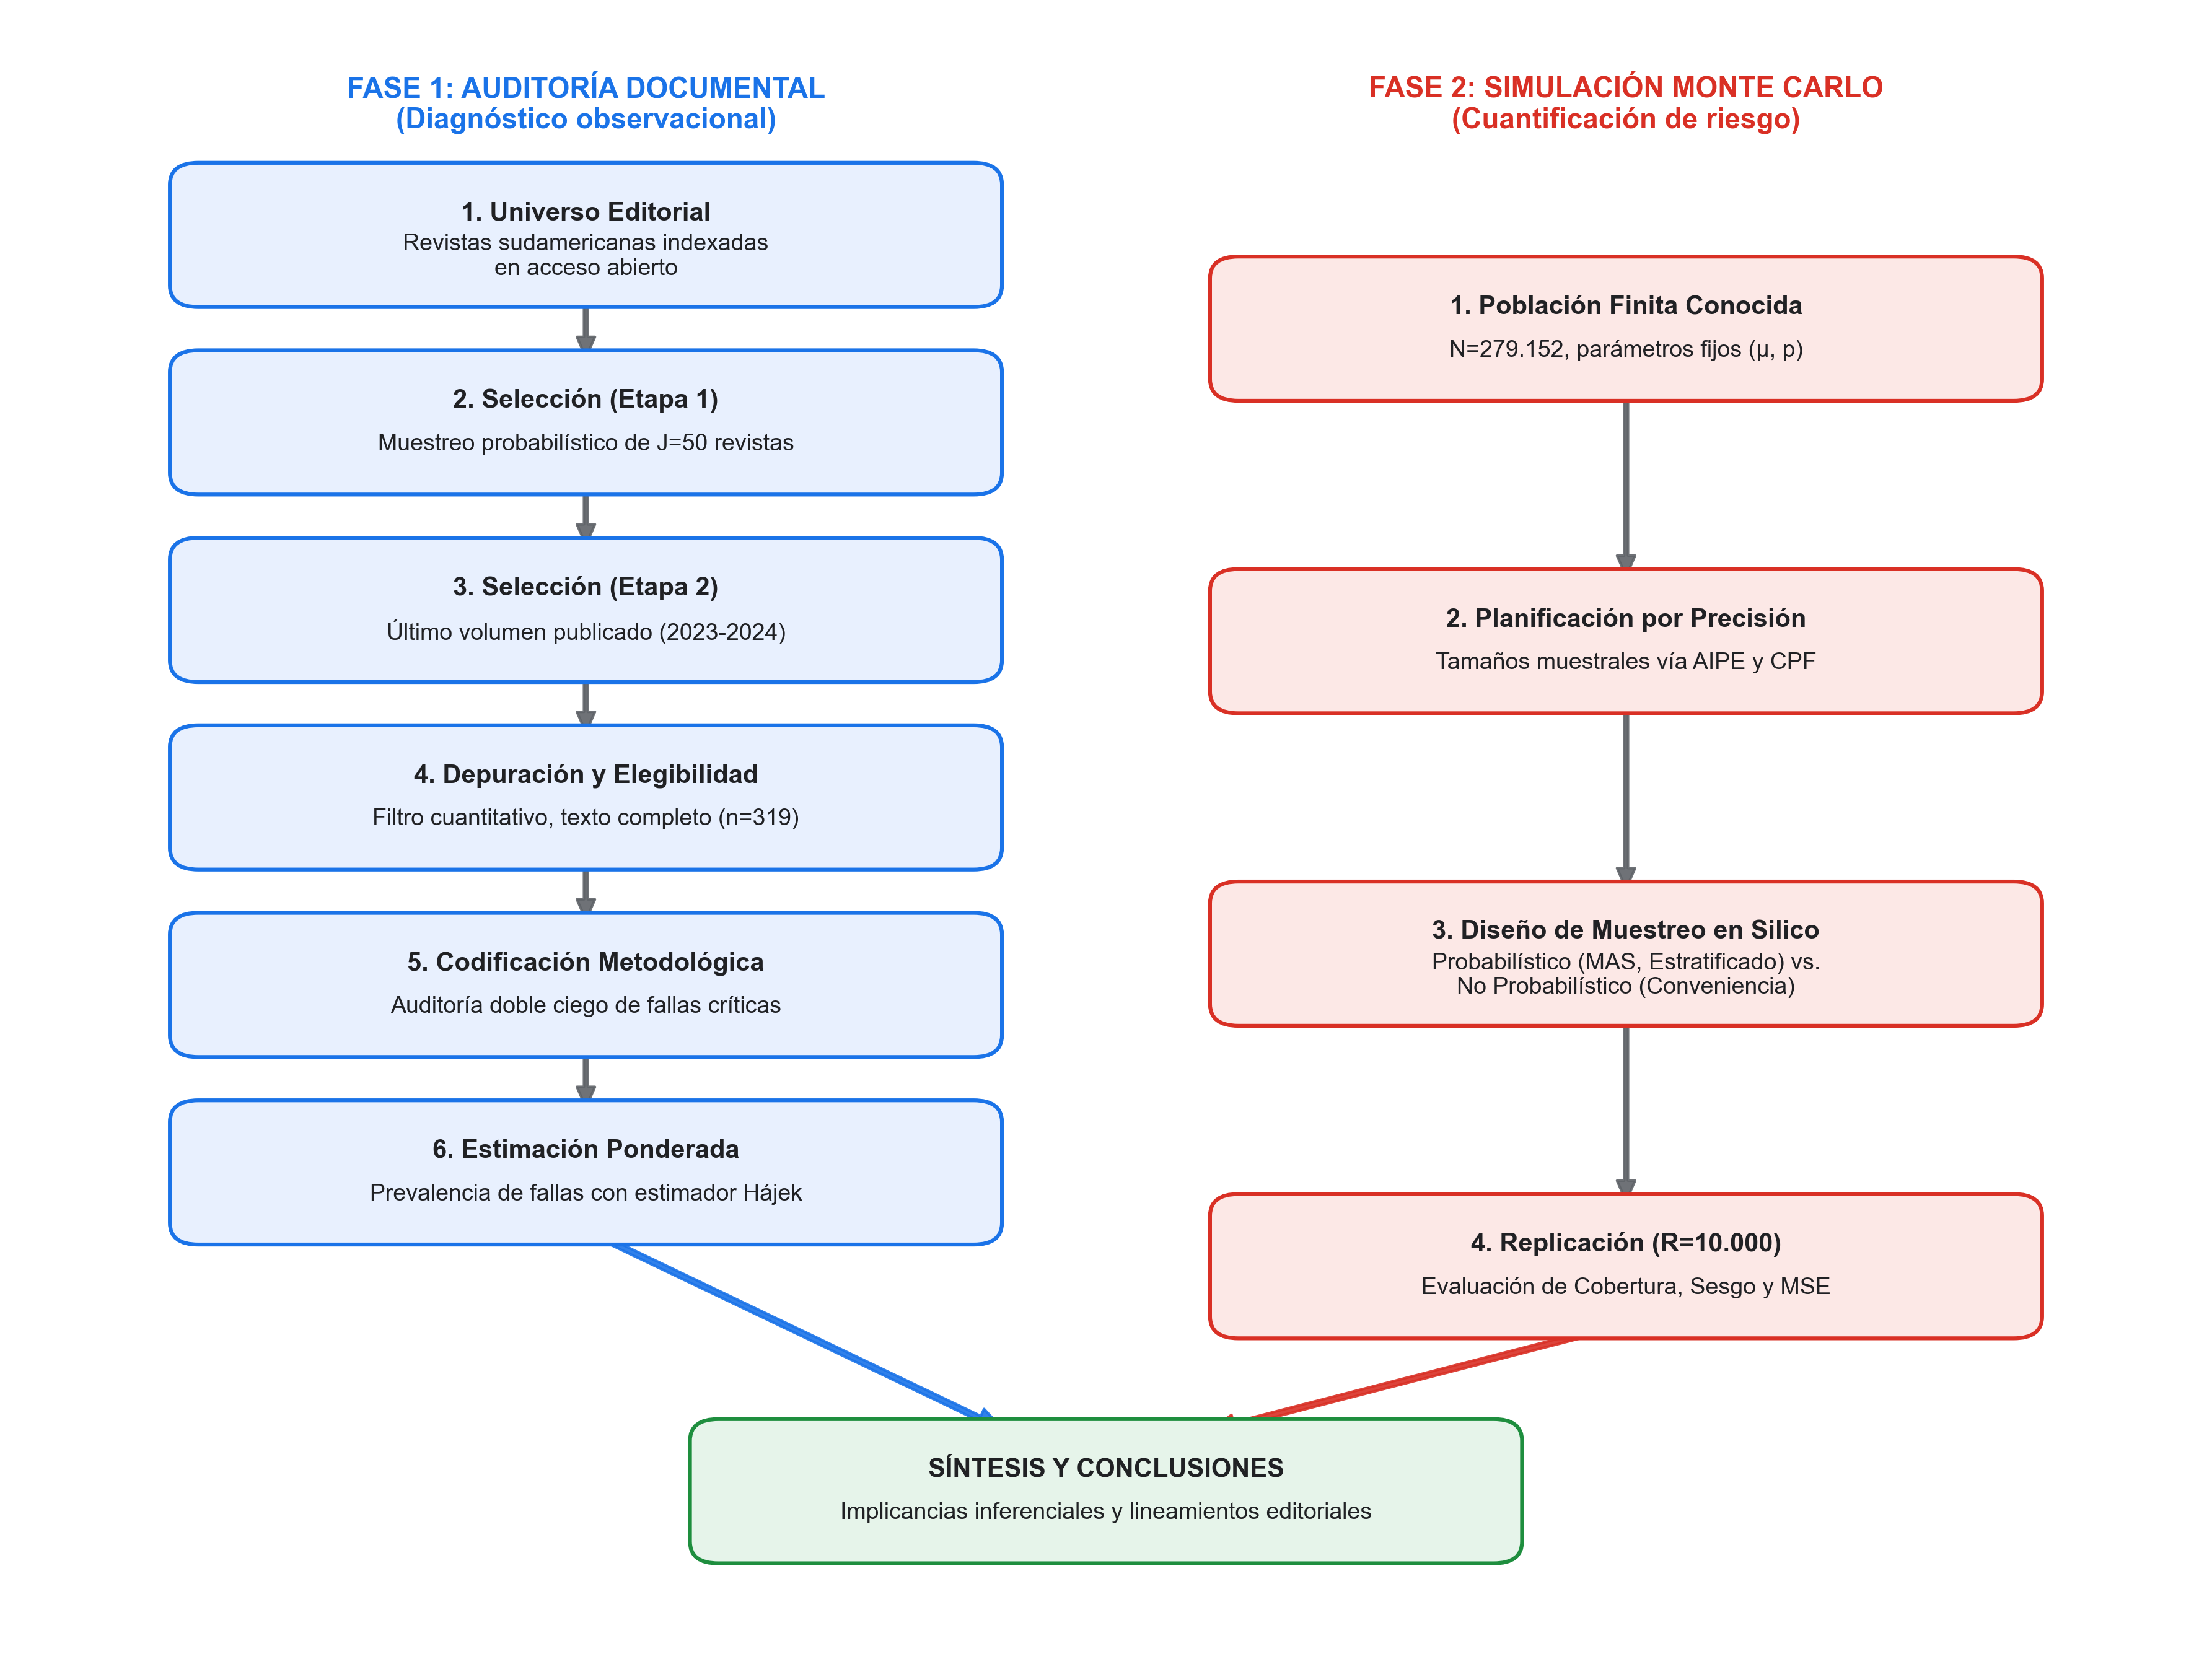
\includegraphics[width=\linewidth]{figura_metodologia_dual.png}
\caption{Mapa de síntesis de los procesos metodológicos: construcción del corpus analítico desde el universo DOAJ hasta la base final de 628 artículos. Fuente: Elaboración propia.}
\label{fig:flujo_corpus}
\end{figure}

\subsection{Fase diagnóstica}

El universo objetivo estuvo conformado por revistas sudamericanas de acceso abierto indizadas en el \textit{Directory of Open Access Journals} (DOAJ). Se seleccionaron las revistas con sede editorial en los países de América del Sur, obteniendo un universo operativo inicial. Solo se incluyeron revistas que publican investigaciones con enfoque cuantitativo inferencial o experimental, identificadas mediante los códigos temáticos \textit{Library of Congress Classification} (LCC).

La unidad de análisis estructurante inicial fue la \textbf{revista}, mientras que la unidad analítica final fue el \textbf{artículo}. Se consideraron elegibles artículos originales con metodología cuantitativa o mixta que utilizaran herramientas inferenciales (por ejemplo, pruebas de hipótesis, \IC, modelos de regresión u otros procedimientos estadísticos) procedentes del catálogo de dichas revistas.

Se aplicó un muestreo estratificado proporcional multietápico. En la primera etapa se seleccionaron revistas de forma aleatoria. En la segunda etapa, mediante la consulta automatizada a la API pública de DOAJ (\texttt{/api/search/articles/issn:\{issn\}}), se extrajeron los artículos más recientes de cada publicación seleccionada, priorizando desde el año 2018 al presente, hasta un tope preestablecido por revista. Los archivos en formato PDF de los artículos se recolectaron automáticamente mediante estrategias de descarga (metaetiquetas de OJS, enlaces directos en SciELO o Redalyc). En el último ciclo de expansión, se conformó una muestra final analizable de 2\,191 artículos, de los cuales 628 utilizaron efectivamente estadística inferencial y constituyeron la base analítica.

El texto de cada PDF fue extraído mediante la biblioteca \texttt{pdfplumber} y analizado con el motor \textit{Gemini 2.5 Flash} (Google DeepMind). Para ello se construyó un canal de extracción automatizada con validación formal JSON mediante el estándar Pydantic. Las variables estructuradas recuperadas por el modelo incluyeron disciplina, tipo de estudio, justificación de diseño, tamaño muestral y tipo de muestreo declarado, uso efectivo de inferencia, extrapolación a la población y el reporte de advertencias sobre limitaciones.

La variable resultado principal fue el indicador de falla inferencial estricta. Históricamente analizado de manera binaria, el diseño actual lo estratificó en tres categorías para ofrecer mayor sensibilidad diagnóstica. El evento de interés analizado empíricamente corresponde a la categoría de \textbf{Falla fuerte}, definida cuando se cumplen simultáneamente tres condiciones: el artículo aplica estadística inferencial (pruebas de hipótesis, \pvalue, regresión) o extrapola resultados a la población; la muestra documentada es de carácter no probabilístico (conveniencia, bola de nieve, intencional); y el artículo omite reportar y advertir explícitamente esta limitación originaria.

Otras clasificaciones producidas incluyen las \textit{Debilidades importantes} (inferencia sobre muestras no probabilísticas pero con un descargo o advertencia autoral visible) y los casos \textit{Sin falla relevante} (inferencia aplicada rigurosamente bajo esquemas probabilísticos consistentes). En este estudio, la tasa de prevalencia reportada se centró exclusivamente en documentar la Falla Fuerte como un incumplimiento rotundo a nivel de artículo individual. Se omite explícitamente la derivación de estimadores de prevalencia a nivel de revista. Esto se fundamenta en la naturaleza heterogénea de muchas publicaciones multidisciplinarias, donde coexisten artículos con legítimo alcance descriptivo y cualitativo junto con aquellos que aplican inferencia de manera problemática, haciendo geométricamente ambiguo el clasificar toda una revista bajo una única categorización dicotómica.

A nivel artículo, el estimando objetivo fue la prevalencia poblacional de artículos cuantitativos que cometen una \textit{Falla fuerte}:
\[
P_A=\frac{1}{N_A}\sum_{i=1}^{N_A} y_{i},
\]
donde $y_{i} \in \{0,1\}$ indica la existencia de Falla Fuerte en el artículo $i$, y $N_A$ la muestra de artículos que aplican inferencia estadística. Las prevalencias empíricas fueron analizadas mediante estratos por macroárea disciplinar y país de origen, contrastando la independencia de distribuciones a través de pruebas paramétricas como $\chi^2$.

La planificación por precisión mantuvo el marco de \textit{accuracy in parameter estimation} (AIPE) como criterio fundacional de planificación poblacional \citep{noordzij2010}. Para proporciones inferenciales simuladas:
\[
n_0=\frac{z_{1-\alpha/2}^2 p(1-p)}{d^2}, \qquad n=\frac{n_0}{1+\frac{n_0-1}{N}}.
\]
Con base en una precisión objetivo de $\pm 5$\,puntos porcentuales y un escenario conservador ($p=0{,}5$), la recomendación empírica fue de aproximadamente 385 a $400$ unidades. La expansión final a $n=628$ artículos cuantitativos evaluables provee certidumbre suficiente para estabilizar los intervalos de confianza en el análisis descriptivo transversal.

\subsection{Fase de simulación}

La simulación se construyó sobre una población finita de referencia de tamaño $N=279.152$. Los parámetros verdaderos fijados para el experimento fueron una proporción $p=0{,}524$, una media $\mu=7.077.586$~Gs y un desvío estándar $\sigma=5.153.750$~Gs. Estos valores fueron calibrados para una población sintética verosímil con el perfil sociodemográfico y distributivo de referencia presentado en la Tabla~\ref{tab:parametros_sim}, y se utilizaron únicamente como referencia computacional para evaluar desempeño inferencial; no corresponden a una población observada específica. Se fijaron además $R=10.000$ réplicas Monte Carlo, nivel de confianza de 95\,\%, valor crítico $z=1{,}95996$, margen de error objetivo $d_{prop}=0{,}05$ para proporciones y $d_{\mu}=300.000$~Gs para medias.

Se compararon tres mecanismos de selección: la selección aleatoria simple sin reposición (\SRS); el estratificado proporcional, con asignación por estratos en proporción a su tamaño poblacional; y la conveniencia, modelada como un mecanismo no probabilístico mediante selección endógena dependiente de características asociadas con la variable de interés. La regla de conveniencia se definió explícitamente para que la inclusión no fuera independiente del resultado, reproduciendo un escenario plausible de sesgo de selección. Precisamente por esa razón, la cobertura poblacional de los intervalos bajo conveniencia no se interpretó como una métrica válida.

Para cada réplica $r$, se calcularon estimadores de proporción y media. El desempeño se resumió mediante sesgo relativo, \RMSE\ y cobertura empírica en los diseños probabilísticos:
\[
\widehat{\mathrm{Bias}}(\widehat{\theta})=\frac{1}{R}\sum_{r=1}^{R}\widehat{\theta}^{(r)}-\theta,
\]
\[
\sesgorel(\widehat{\theta})=
100\cdot\frac{\widehat{\mathrm{Bias}}(\widehat{\theta})}{\theta},
\qquad
\RMSE(\widehat{\theta})=
\sqrt{\frac{1}{R}\sum_{r=1}^{R}\left(\widehat{\theta}^{(r)}-\theta\right)^2}.
\]
La cobertura se definió como
\[
\widehat{\mathrm{Cov}}=\frac{1}{R}\sum_{r=1}^{R}\mathbb{I}\left(\theta\in \IC^{(r)}\right).
\]

El bootstrap se utilizó solo como diagnóstico numérico de variabilidad condicional a la muestra. En ningún caso se interpretó como mecanismo capaz de restaurar validez inferencial poblacional cuando la muestra madre fue obtenida por conveniencia. Los intervalos bootstrap se reportan, por tanto, exclusivamente como medida de estabilidad interna y no como cobertura poblacional \citep{noordzij2010,reinhart2015}.

\section{Resultados}
\label{sec:resultados}

La base final estuvo conformada por 628 artículos que aplican estadística inferencial procedentes de las descargas en repositorios regionales. La recolección automatizada y el filtro de elegibilidad mediante extracción por IA permitieron recuperar de manera eficiente el corpus, cuya construcción exhaustiva se describió en la Sección~\ref{sec:metodologia}. A la luz del nuevo diseño, las prevalencias y resultados se reportan exclusivamente a nivel de unidad analítica primaria (el artículo).

A nivel general, el 39,0\,\% de los artículos analizados ($n=245$ de 628) incurrió en una \textbf{Falla Fuerte}, definida por la aplicación iterativa de estadística inferencial sobre marcos muestrales de conveniencia sin advertir explícita o discutir dicha limitación durante el reporte de resultados. Un 49,7\,\% adicional ($n=312$) aplicó la misma mecánica inferencial pero adjuntando una declaración de limitante explícita (clasificada metodológicamente como \textit{Debilidad Importante}). Apenas el 11,3\,\% ($n=71$) de la muestra evidenció rigor completo y se ubicó en la categoría de \textit{Sin Falla Relevante}.

Estas métricas ilustran de manera contundente un problema estructural de la literatura empírica auditada: acumulativamente, un 88,7\,\% de los artículos aplica un andamiaje inferencial estadísticamente desanclado de un marco poblacional probabilístico.

La distribución según áreas de encuadramiento expone marcados matices empíricos. Según los indicadores estructurales, las Ciencias de la Educación seguidas de las Ciencias Naturales presentan las mayores prevalencias en la categoría de \textit{Fallas Fuertes} (superiores al 42\,\%). En contrapartida, las Ciencias de la Salud exponen la mayor porción de \textit{Debilidades Importantes} (63,9\,\%), donde la mayoría de los investigadores procede a realizar la generalización estadística no probabilística acompañándola con exenciones discursivas.

\begin{figure}[H]
\centering
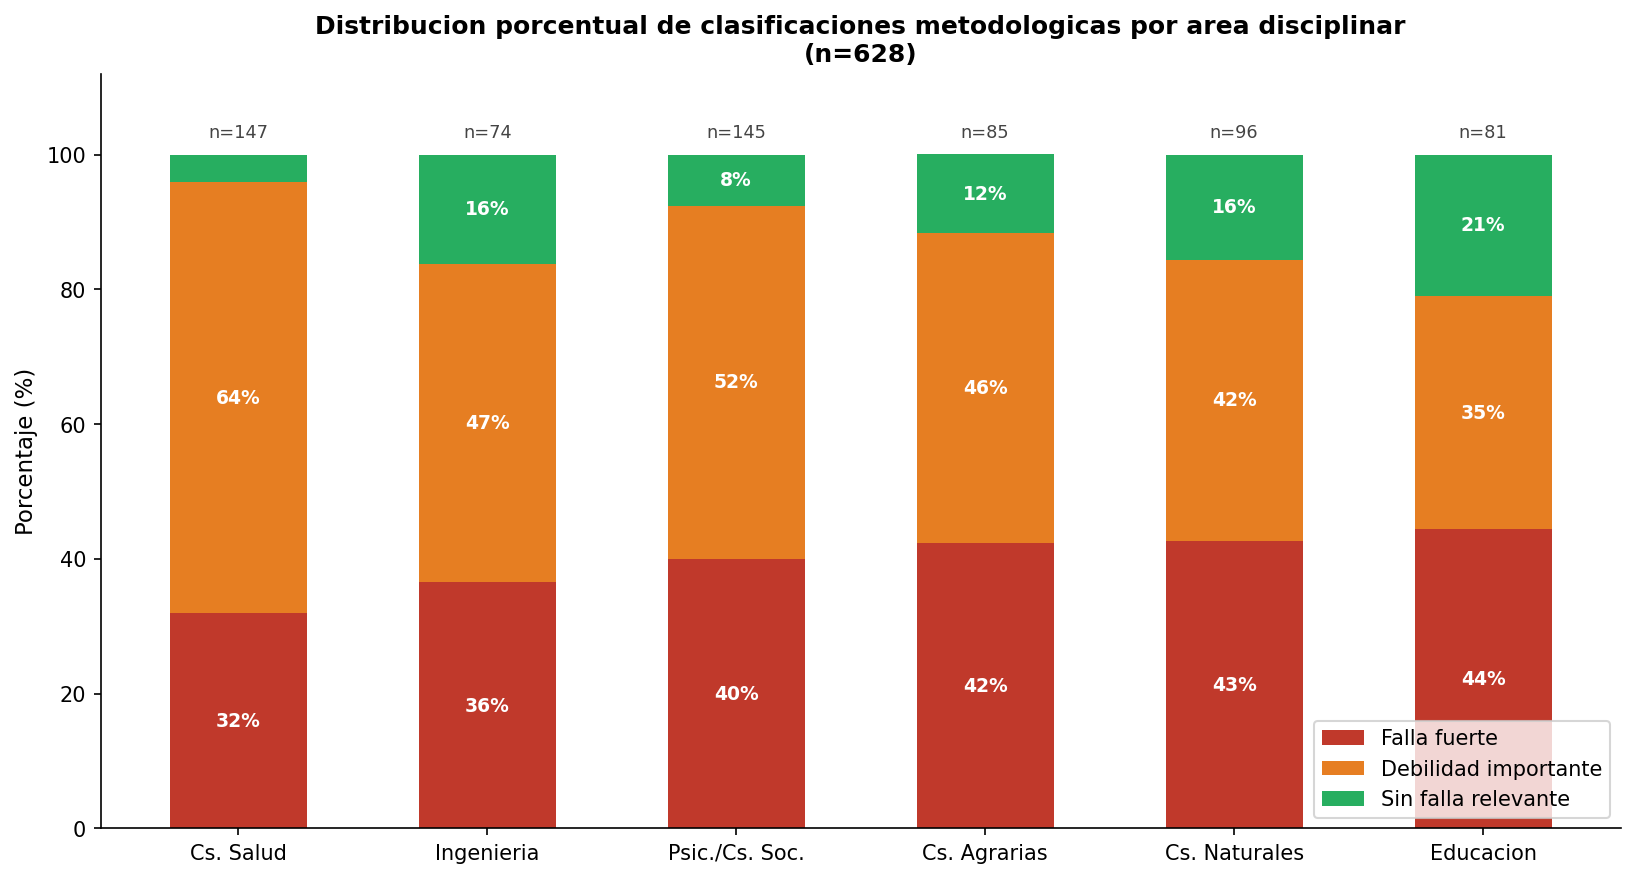
\includegraphics[width=\linewidth]{fig2_distribucion_porcentual_por_area.png}
\caption{Distribución porcentual de las categorías de falla según macroárea disciplinar. Fuente: Elaboración propia a partir de datos de DOAJ.}
\label{fig:distribucion_porcentual}
\end{figure}

El desglose volumétrico de los artículos evaluados puede consultarse en la Tabla~\ref{tab:distribucion_area}.

\begin{table}[H]
\centering
\caption{Distribución absoluta y porcentual por categoría y área disciplinar.}
\label{tab:distribucion_area}
\begin{tabular}{lrrrrrrr}
\toprule
\textbf{Área} & \textbf{FF} & \textbf{DI} & \textbf{SFR} & \textbf{TOTAL} & \textbf{\%FF} & \textbf{\%DI} & \textbf{\%SFR} \\
\midrule
Cs. Salud & 47 & 94 & 6 & 147 & 32.0 & 63.9 & 4.1 \\
Cs. Naturales & 41 & 40 & 15 & 96 & 42.7 & 41.7 & 15.6 \\
Cs. Agrarias & 36 & 39 & 10 & 85 & 42.4 & 45.9 & 11.8 \\
Psic./Cs. Soc. & 58 & 76 & 11 & 145 & 40.0 & 52.4 & 7.6 \\
Ingenieria & 27 & 35 & 12 & 74 & 36.5 & 47.3 & 16.2 \\
Educacion & 36 & 28 & 17 & 81 & 44.4 & 34.6 & 21.0 \\
\textbf{TOTAL} & \textbf{245} & \textbf{312} & \textbf{71} & \textbf{628} & \textbf{39.0} & \textbf{49.7} & \textbf{11.3} \\
\bottomrule
\end{tabular}
\begin{flushleft}
\footnotesize Fuente: Elaboración propia a partir de datos de DOAJ. Nota: FF = Falla Fuerte; DI = Debilidad Importante; SFR = Sin Falla Relevante. Elaboración estructural sobre $n=628$ artículos.
\end{flushleft}
\end{table}

Los artículos auditados cubren el período 2018--2025, lo que refleja la producción científica más reciente del ecosistema regional.

En cuanto a la fase de simulación, la Tabla~\ref{tab:parametros_sim} resume los parámetros fijos del experimento Monte Carlo. Estos valores se utilizaron como referencia de una población finita sintética calibrada y no deben interpretarse como estimaciones sustantivas para una población observada particular.

\begin{table}[H]
\centering
\caption{Parámetros de ejecución y parámetros de referencia utilizados en la simulación.}
\label{tab:parametros_sim}
\begin{tabular}{lr}
\toprule
\textbf{Parámetro} & \textbf{Valor} \\
\midrule
Réplicas Monte Carlo ($R$) & 10.000 \\
Nivel de confianza & 95\,\% \\
Valor crítico $z$ & 1,95996 \\
Margen de error para proporción ($d_{prop}$) & 0,05 \\
Margen de error para media ($d_{\mu}$) & 300.000 Gs \\
Tamaño poblacional ($N$) & 279.152 \\
Proporción verdadera ($p$) & 0,524 \\
Media verdadera ($\mu$) & 7.077.586 Gs \\
Desvío estándar ($\sigma$) & 5.153.750 Gs \\
\bottomrule
\end{tabular}
\begin{flushleft}
\footnotesize Fuente: Elaboración propia.
\end{flushleft}
\end{table}

La Tabla~\ref{tab:n_objetivo} muestra los tamaños muestrales requeridos con y sin \CPF. Dado el tamaño poblacional de referencia, la \CPF\ tuvo un efecto marginal.

\begin{table}[H]
\centering
\caption{Tamaños muestrales requeridos con y sin corrección por población finita.}
\label{tab:n_objetivo}
\begin{tabular}{lrr}
\toprule
\textbf{Estimando} & \textbf{$n$ sin \CPF} & \textbf{$n$ con \CPF} \\
\midrule
Proporción & 385 & 384 \\
Media & 1.134 & 1.130 \\
\bottomrule
\end{tabular}
\begin{flushleft}
\footnotesize Fuente: Elaboración propia.
\end{flushleft}
\end{table}

La Tabla~\ref{tab:sensibilidad_cpf} ilustra el comportamiento de \CPF\ bajo diferentes tamaños poblacionales y valores de $p$. Para proporciones, el tamaño depende de $p(1-p)$, por lo que los escenarios $p=0{,}2$ y $p=0{,}8$ son simétricos.

\begin{table}[H]
\centering
\caption{Sensibilidad del tamaño muestral para proporción a $N$ y $p$, con y sin \CPF.}
\label{tab:sensibilidad_cpf}
\begin{tabular}{rrrrr}
\toprule
\textbf{$N$} & \textbf{$p$} & \textbf{$n$ sin \CPF} & \textbf{$n$ con \CPF} & \textbf{Reducción (\%)} \\
\midrule
1.000 & 0,2 & 246 & 198 & 19,5 \\
10.000 & 0,2 & 246 & 240 & 2,4 \\
279.152 & 0,2 & 246 & 246 & 0,0 \\
1.000 & 0,5 & 385 & 278 & 27,8 \\
10.000 & 0,5 & 385 & 370 & 3,9 \\
279.152 & 0,5 & 385 & 384 & 0,3 \\
1.000 & 0,8 & 246 & 198 & 19,5 \\
10.000 & 0,8 & 246 & 240 & 2,4 \\
279.152 & 0,8 & 246 & 246 & 0,0 \\
\bottomrule
\end{tabular}
\begin{flushleft}
\footnotesize Fuente: Elaboración propia. Nota: Para proporciones, el tamaño muestral depende de $p(1-p)$; por ello, $p=0{,}2$ y $p=0{,}8$ son simétricos.
\end{flushleft}
\end{table}

La Tabla~\ref{tab:sim_prob} resume cobertura, sesgo relativo y \RMSE\ bajo \SRS\ y estratificación proporcional. En ambos diseños la cobertura se mantuvo próxima a la nominal, con sesgo bajo y \RMSE\ acotado.

\begin{table}[H]
\centering
\caption{Desempeño inferencial bajo diseños probabilísticos.}
\label{tab:sim_prob}
\begin{tabular}{lrrr}
\toprule
\textbf{Diseño y parámetro} & \textbf{Cobertura (\%)} & \textbf{Sesgo (\%)} & \textbf{\RMSE} \\
\midrule
\SRS, proporción & 95 & 0,73 & 0,025 \\
\SRS, media (Gs) & 93 & -0,31 & 143.848 \\
Estratificado proporcional, proporción & 95 & -0,42 & 0,024 \\
Estratificado proporcional, media (Gs) & 96 & -0,12 & 140.326 \\
\bottomrule
\end{tabular}
\begin{flushleft}
\footnotesize Fuente: Elaboración propia. Nota: La cobertura se reporta solo para diseños probabilísticos.
\end{flushleft}
\end{table}

Bajo conveniencia no se reportó cobertura poblacional, porque el mecanismo de inclusión depende del proceso de selección y rompe la base probabilística que sustenta la interpretación frecuentista del intervalo. En este escenario se reportaron solo sesgo relativo y \RMSE.

\begin{table}[H]
\centering
\caption{Desempeño bajo muestreo por conveniencia.}
\label{tab:sim_conv}
\begin{tabular}{lrr}
\toprule
\textbf{Parámetro} & \textbf{Sesgo (\%)} & \textbf{\RMSE} \\
\midrule
Proporción & 2,51 & 0,027 \\
Media (Gs) & 2,10 & 198.422 \\
\bottomrule
\end{tabular}
\begin{flushleft}
\footnotesize Fuente: Elaboración propia. Nota: No se reporta cobertura porque el mecanismo de selección por conveniencia impide interpretación poblacional del \IC.
\end{flushleft}
\end{table}

La fase diagnóstica mostró una prevalencia sustantiva de fallas inferenciales críticas y un gradiente claro según tipo de muestreo. La fase de simulación confirmó que, cuando el mecanismo de selección es probabilístico, la cobertura se aproxima a la nominal; en cambio, bajo conveniencia se observa sesgo estructural y pérdida de interpretabilidad inferencial.

En conjunto, ambos componentes convergen en un mismo punto: la validez de la inferencia no depende solo del estimador o del software utilizado, sino de la coherencia entre población objetivo, mecanismo de selección, cálculo de tamaño muestral, estimación de varianza e interpretación final.

La Figura~\ref{fig:simulacion_mc} sintetiza visualmente los tres criterios de desempeño evaluados.

\begin{figure}[H]
\centering
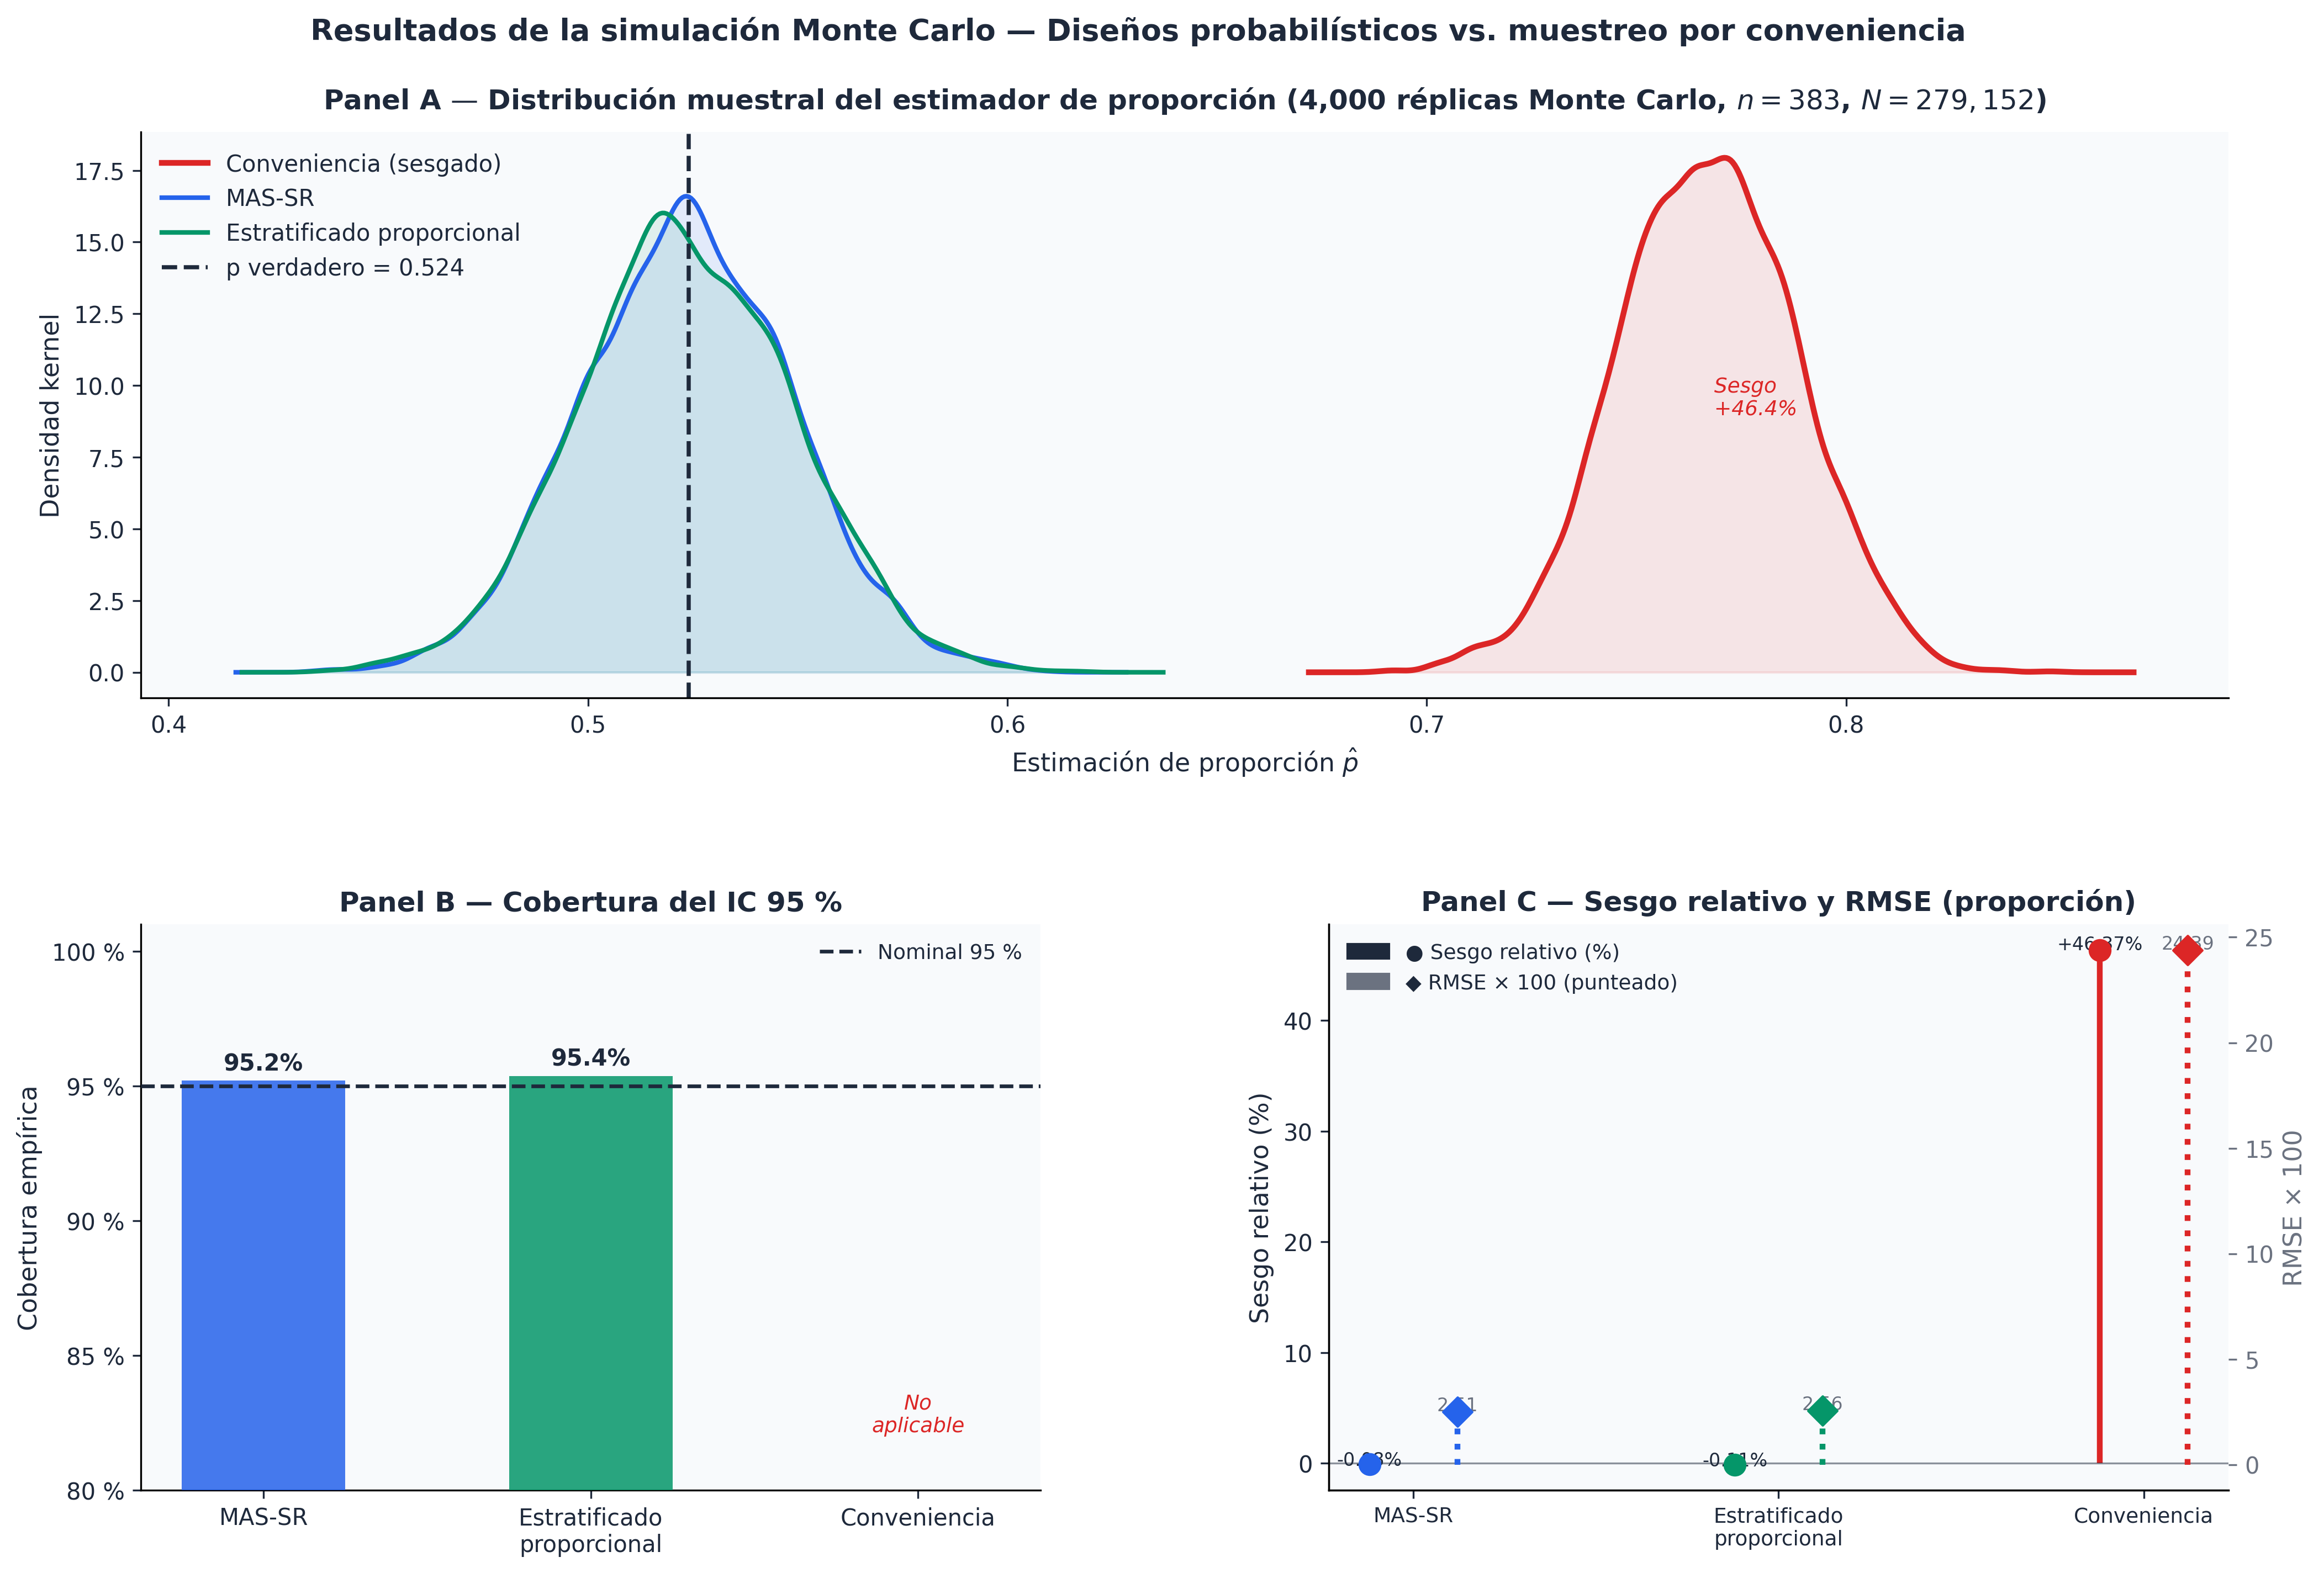
\includegraphics[width=\linewidth]{fig_simulacion_resultados.png}
\caption{Resultados de la simulación Monte Carlo ($R=10\,000$ réplicas, $N=279\,152$, $n=384$ para proporciones con \CPF).
\textbf{Panel~A}: distribución muestral del estimador $\hatP$ para los tres diseños;
las curvas del \SRS\ y del estratificado se superponen sobre el valor verdadero $p=0{,}524$,
mientras que la conveniencia exhibe desplazamiento sistemático.
\textbf{Panel~B}: cobertura empírica del \IC\ 95\,\%; la línea discontinua indica el nivel nominal.
\textbf{Panel~C}: sesgo relativo (\%) y \RMSE\ por diseño; los diseños probabilísticos
presentan sesgo cercano a cero y \RMSE\ similar, en contraste con la conveniencia. Fuente: Elaboración propia.}
\label{fig:simulacion_mc}
\end{figure}

\section{Consideraciones finales}
\label{sec:consideraciones}

La auditoría documental mostró una prevalencia importante de fallas inferenciales críticas en artículos cuantitativos de revistas sudamericanas de acceso abierto. La comparación directa con estudios previos debe hacerse con cautela porque las unidades de análisis, los criterios de codificación y los dominios temáticos no son idénticos. Sin embargo, nuestros hallazgos son consistentes con la literatura que documenta deficiencias persistentes de reporte y de interpretación estadística en múltiples disciplinas \citep{ioannidis2005,darrigo2024,schmidt2025}.

Inéditamente, la prevalencia estricta de \textit{Fallas Fuertes} alcanzó el 39,0\,\% de los artículos empíricos con inferencia encuestados, mientras que una proporción todavía mayor (49,7\,\%) incurrió en procedimientos similares escudados tras una advertencia de limitación. Sumadas, casi 9 de cada 10 manuscritos exhiben incongruencias metodológicas-inferenciales, lo que representa una prevalencia notablemente superior a los rangos reportados en auditorías previas de calidad en otras regiones. Aunque la heterogeneidad de criterios hace improcedente la comparación unívoca, los hallazgos de \citet{schmidt2025} sobre el mal uso del valor $p$ sugieren que este orden de magnitud no es atípico bajo definiciones estrictas de \textit{falla inferencial}.

Un antecedente regional útil es el estudio de \citet{peralta2023}, el cual evaluó artículos de revistas y reportó cumplimientos altos de criterios APA. Aunque ese estudio se enfoca en calidad general de formato, resulta ilustrativo porque sugiere que una estructura formal aceptable no garantiza ninguna correspondencia con el rigor inferencial: un artículo puede estar bien formateado y aun así presentar problemas severos de muestreo, extrapolación e interpretación.

A nivel internacional, la literatura sobre lineamientos editoriales también ha mostrado vacíos recurrentes en el reporte de elementos esenciales \citep{schulz2010}. Si bien esto se conoce en ensayos clínicos, nuestro estudio refuerza la idea de que omisiones de diseño y precisión permeabilizan todo el abanico disciplinario, afectando desde Ciencias de la Salud hasta Ciencias Exactas, Naturales y Educación.

Una contribución central del estudio es metodológica. Al transitar hacia la recuperación y clasificación documental asistida por Inteligencia Artificial y confirmación humana, incrementos exponenciales en los volúmenes de revisión ---llegando a más de 600 artículos con clasificación integral--- se hacen posibles, reduciendo la dependencia sobre muestras pequeñas de conveniencia. Asimismo, la definición explícita de falla inferencial estricta como un problema rotundo (\textit{Falla Fuerte}) elimina ambigüedades. El protocolo diferenció penalizaciones por desconocimiento total frente a debilidades declaradas, lo cual añade densidad al debate sobre si basta con justificar una debilidad metodológica para continuar esgrimiendo pruebas inferenciales con aparente normalidad.

La fase de simulación permitió separar con claridad dos planos. En el plano probabilístico, \SRS\ y la estratificación proporcional produjeron coberturas próximas a la nominal, junto con sesgos reducidos y \RMSE\ acotado. En el plano no probabilístico, la selección por conveniencia generó sesgo estructural y volvió improcedente la interpretación de cobertura poblacional. Este resultado es coherente con la literatura metodológica. Las fórmulas de tamaño muestral y los \IC\ clásicos suponen un mecanismo probabilístico de selección, por lo que su traslado automático a muestras de conveniencia carece de justificación \citep{noordzij2010}. Del mismo modo, las advertencias sobre el uso de poder post-hoc, inferencia desanclada del diseño y reexpresiones numéricas de la incertidumbre sin base probabilística apuntan en la misma dirección \citep{hoenig2001,thomas1997,reinhart2015,navarrete2019}. Nuestra simulación no pretende resolver un debate teórico abierto, sino mostrar cuantitativamente que, bajo el mecanismo de conveniencia modelado, el sesgo persiste aunque se apliquen procedimientos de remuestreo.

Por esa razón, el bootstrap se interpretó solo como diagnóstico de variabilidad condicional a la muestra. Este punto es importante porque en la práctica aplicada suele utilizarse como sustituto informal de la aleatorización. Nuestros resultados muestran que, en los escenarios evaluados, el remuestreo no corrige la incoherencia originaria entre diseño de selección y validez inferencial.

La pertinencia regional del estudio radica en que el ecosistema sudamericano de acceso abierto combina diversidad disciplinaria, multilingüismo y modelos editoriales con recursos heterogéneos \citep{beigel2024}. En ese contexto, las exigencias estadísticas suelen ser menos visibles que las exigencias formales de estilo o estructura. Nuestros hallazgos sugieren que la mejora editorial no depende solo de reforzar normas generales de presentación, sino de exigir información mínima sobre población objetivo, marco muestral, mecanismo de selección, pesos, varianza y alcance de la inferencia. Los hallazgos del estudio sugieren que las revistas no deberían limitar la evaluación metodológica a la presencia de pruebas estadísticas o a la estructura formal del manuscrito. La revisión editorial debe verificar coherencia entre población objetivo, mecanismo de selección, estimador, método de varianza e interpretación. Esta recomendación es consistente con el espíritu de STROBE, CONSORT y SAMPL, pero aquí se operacionaliza en una herramienta breve orientada a la coherencia inferencial \citep{vonelm2007,schulz2010,lang2015}. El Apéndice~\ref{app:checklist} presenta un checklist mínimo que traduce estos principios en preguntas concretas y verificables, susceptible de integrarse a las instrucciones para autores, a formularios de revisión por pares o a listas internas de control editorial.

El estudio presenta, no obstante, varias limitaciones que deben explicitarse. En primer lugar, el marco editorial puede presentar subcobertura si existen revistas sudamericanas pertinentes fuera de las fuentes utilizadas para construir el universo. En segundo término, la clasificación del tipo de muestreo depende del reporte disponible en los artículos, por lo que es posible cierta misclasificación cuando los autores describen de forma incompleta el mecanismo real de selección. En tercer lugar, algunos subgrupos son pequeños, en especial el idioma inglés, por lo que los resultados estratificados deben interpretarse de manera descriptiva. Finalmente, la fase de simulación representa un mecanismo específico de conveniencia; otras formas de selección no probabilística podrían producir magnitudes distintas de sesgo y \RMSE.

Entre las líneas futuras de investigación, resulta particularmente relevante ampliar el marco editorial a otras bases y actualizar la auditoría de forma longitudinal; estimar prevalencias por categoría específica de falla, además del indicador compuesto; incorporar no respuesta y mecanismos de selección más complejos en la simulación; y evaluar el efecto de políticas editoriales o checklists estadísticos sobre la prevalencia de fallas a lo largo del tiempo.

En relación con auditorías previas, este estudio aporta un diagnóstico con diseño probabilístico, ponderación e \IC\ basados en varianza de diseño. En relación con la literatura sobre muestreo no probabilístico, aporta una demostración cuantitativa de la pérdida de validez inferencial bajo conveniencia en los escenarios evaluados. En relación con las guías editoriales, aporta una traducción operativa de sus principios hacia un checklist centrado en población, selección, precisión, varianza e interpretación.

El patrón observado no se reduce a errores aislados de redacción, sino que expresa una desconexión más profunda entre población objetivo, mecanismo de selección, cálculo de tamaño muestral, estimación de varianza e interpretación final. En términos prácticos, el aporte del estudio es doble. Por un lado, ofrece un diagnóstico con base de diseño sobre la prevalencia de fallas inferenciales críticas. Por otro, propone una herramienta editorial breve para fortalecer la coherencia entre diseño, análisis e interpretación. Ambos aportes convergen en una misma conclusión: mejorar la calidad de la investigación cuantitativa requiere pasar de un énfasis exclusivo en significancia y formato a un estándar explícito de transparencia metodológica y precisión inferencial.


% Apéndice (opcional)
\appendix

\section{Reglas resumidas de codificación de fallas inferenciales críticas}
\label{app:codificacion}

\begin{longtable}{P{4.0cm}P{5.1cm}P{5.6cm}}
\caption{Protocolo resumido de codificación.}
\label{tab:protocolo_codificacion}\\
\toprule
\textbf{Categoría} & \textbf{Evidencia buscada} & \textbf{Regla de codificación} \\
\midrule
\endfirsthead
\toprule
\textbf{Categoría} & \textbf{Evidencia buscada} & \textbf{Regla de codificación} \\
\midrule
\endhead
No significancia interpretada como ausencia de efecto & Frases que concluyen ``no hay efecto'', ``no existe asociación'' o equivalentes a partir de un resultado no significativo, sin considerar \IC\ o umbrales de relevancia. & Se codifica falla si la conclusión excede lo permitido por la incertidumbre reportada. \\
Comparación incorrecta entre grupos & Afirmaciones del tipo ``un grupo fue significativo y el otro no, por lo tanto son diferentes'', sin contraste directo entre estimadores. & Se codifica falla si la comparación entre grupos no se basa en el parámetro de diferencia pertinente. \\
Poder post-hoc como justificación & Cálculo de poder retrospectivo con el efecto observado para justificar validez o suficiencia de la muestra. & Se codifica falla cuando el poder post-hoc se presenta como validación sustantiva del estudio. \\
Inferencia en censo completo sin superpoblación & Uso de \pvalue, \IC\ o lenguaje inferencial sobre un censo completo sin definir modelo generador o superpoblación. & Se codifica falla cuando no existe justificación explícita para inferencia más allá de la población observada. \\
Incoherencia diseño-inferencia & Cálculo o lenguaje inferencial probabilístico aplicado a muestras de conveniencia o selección no probabilística, sin justificación clara. & Se codifica falla cuando los supuestos del análisis son incompatibles con el mecanismo real de selección. \\
Ausencia de población o marco muestral & El artículo no define población objetivo, unidad de selección o marco muestral. & Se codifica falla cuando la omisión impide evaluar la validez externa del estudio. \\
Reporte incompleto de pesos o varianza & En diseños complejos, el artículo omite pesos, estratos, conglomerados o método de varianza. & Se codifica falla cuando el lector no puede reconstruir la base del error estándar o del \IC. \\
\bottomrule
\end{longtable}

\begin{flushleft}
\footnotesize Fuente: Elaboración propia.
\end{flushleft}

\section{Detalle conceptual del escenario de conveniencia modelado}
\label{app:conveniencia_modelada}

El mecanismo de conveniencia utilizado en la simulación se definió como un proceso de inclusión no probabilística dependiente de características asociadas con la variable de interés. Su propósito fue representar un escenario plausible de captación dirigida y no un inventario exhaustivo de todas las formas de selección no probabilística.

Las implicancias de este diseño son directas: la probabilidad de inclusión deja de ser conocida y distinta de cero para todas las unidades; el sesgo de selección afecta el centro de la distribución muestral, no solo su dispersión; un \IC\ construido bajo supuestos probabilísticos pierde interpretación de cobertura poblacional; y el bootstrap puede describir variabilidad interna de la muestra observada, pero no restaurar la propiedad de aleatorización ausente en el diseño original.

\section{Checklist mínimo para evaluación editorial}
\label{app:checklist}

\begin{longtable}{P{2.1cm}P{3.3cm}P{6.0cm}P{4.1cm}}
\caption{Checklist mínimo para evaluación editorial de coherencia inferencial.}
\label{tab:checklist}\\
\toprule
\textbf{Prioridad} & \textbf{Ítem mínimo} & \textbf{Qué debe reportarse} & \textbf{Motivo} \\
\midrule
\endfirsthead
\toprule
\textbf{Prioridad} & \textbf{Ítem mínimo} & \textbf{Qué debe reportarse} & \textbf{Motivo} \\
\midrule
\endhead
Obligatorio & Población y marco & Población objetivo, unidad de análisis, unidad de selección y marco muestral o listado de referencia. & Delimita el alcance de la validez externa. \\
Obligatorio & Mecanismo de selección & Si la selección fue probabilística o no probabilística, reglas de inclusión, estratos, conglomerados y etapas de muestreo. & Permite juzgar sesgo de selección e interpretabilidad inferencial. \\
Obligatorio & Tamaño muestral & Justificación del tamaño muestral con nivel de confianza, margen de error, supuestos de variabilidad y, cuando corresponda, \CPF\ y efecto de diseño. & Conecta precisión esperada con diseño y análisis. \\
Obligatorio & Estimador y varianza & Estimador principal, método de error estándar o varianza, uso de pesos y tratamiento de conglomerados o estratos. & Evita \IC\ o pruebas incompatibles con el diseño real. \\
Obligatorio & Criterios de exclusión y no respuesta & Exclusiones, pérdidas, no respuesta y tratamiento analítico de esos casos. & Mejora trazabilidad y reduce sesgos no documentados. \\
Deseable & Subgrupos y multiplicidad & Si los análisis por subgrupos son exploratorios o planificados, y cómo se interpreta su incertidumbre. & Reduce sobrelectura de resultados comparativos. \\
Obligatorio & Datos censales & Si se analizó un censo o la totalidad del marco, aclarar si existe superpoblación o si el análisis es puramente descriptivo. & Evita inferencia injustificada sobre poblaciones completamente observadas. \\
Obligatorio & Interpretación & Discusión basada en magnitud y precisión, no solo en significancia. Debe evitarse interpretar no significancia como ausencia de efecto. & Mejora la calidad de la conclusión sustantiva. \\
Deseable & Remuestreo & Aclarar el objetivo del bootstrap u otros remuestreos y evitar presentarlos como sustitutos de la aleatorización. & Previene interpretaciones erróneas de cobertura poblacional. \\
\bottomrule
\end{longtable}

\begin{flushleft}
\footnotesize Fuente: Elaboración propia.
\end{flushleft}


\newpage
\FloatBarrier
\section*{Referencias}

\begin{thebibliography}{}

\bibitem[Altman y Bland(1995)]{altman1995}
Altman, D.~G. y Bland, J.~M. (1995).
\newblock Statistics notes: absence of evidence is not evidence of absence.
\newblock {\em BMJ}, 311:485.

\bibitem[Beigel et~al.(2024)Beigel, Packer, Gallardo, y Salatino]{beigel2024}
Beigel, F., Packer, A.~L., Gallardo, O., y Salatino, M. (2024).
\newblock OLIVA: La Producción Científica Indexada en América Latina.
\newblock {\em DADOS}, 67(1):e20210174.

\bibitem[D'Arrigo et~al.(2024)D'Arrigo, Abd El Hafeez, Mezzatesta, Abelardo, Provenzano, Vilasi, Torino, y Tripepi]{darrigo2024}
D'Arrigo, G., Abd El Hafeez, S., Mezzatesta, S., Abelardo, D., Provenzano, F.~P., Vilasi, A., Torino, C., y Tripepi, G. (2024).
\newblock Common mistakes in biostatistics.
\newblock {\em Clinical Kidney Journal}, 17(7):sfae197.

\bibitem[Farcomeni(2017)]{farcomeni2017}
Farcomeni, A. (2017).
\newblock Contribution to the discussion of the paper by Stefan Wellek: A critical evaluation of the current p-value controversy.
\newblock {\em Biometrical Journal}, 59(5):1066--1068.

\bibitem[Gelman y Stern(2006)]{gelman2006}
Gelman, A. y Stern, H. (2006).
\newblock The difference between ``significant'' and ``not significant'' is not itself statistically significant.
\newblock {\em The American Statistician}, 60(4):328--331.

\bibitem[Hoenig y Heisey(2001)]{hoenig2001}
Hoenig, J.~M. y Heisey, D.~M. (2001).
\newblock The abuse of power.
\newblock {\em The American Statistician}, 55(1):19--24.

\bibitem[Ioannidis(2005)]{ioannidis2005}
Ioannidis, J.~P.~A. (2005).
\newblock Why most published research findings are false.
\newblock {\em PLoS Medicine}, 2(8):e124.

\bibitem[Lang y Altman(2015)]{lang2015}
Lang, T.~A. y Altman, D.~G. (2015).
\newblock Basic statistical reporting for articles published in biomedical journals: The ``Statistical Analyses and Methods in the Published Literature'' or the {SAMPL} Guidelines.
\newblock {\em International Journal of Nursing Studies}, 52(1):5--9.

\bibitem[Mansournia y Nazemipour(2021)]{mansournia2021}
Mansournia, M.~A. y Nazemipour, M. (2021).
\newblock Recommendations for accurate reporting in medical research statistics.
\newblock {\em The Lancet}, 398(10313):1811.

\bibitem[Navarrete(2019)]{navarrete2019}
Navarrete, M.~S. (2019).
\newblock Ideas equivocadas frecuentes en estadística explicadas sencillamente.
\newblock {\em Medwave}, 19(6):e7660.

\bibitem[Noordzij et~al.(2010)Noordzij, Tripepi, Dekker, Zoccali, Tanck, y Jager]{noordzij2010}
Noordzij, M., Tripepi, G., Dekker, F.~W., Zoccali, C., Tanck, M.~W., y Jager, K.~J. (2010).
\newblock Sample size calculations: basic principles and common pitfalls.
\newblock {\em Nephrology Dialysis Transplantation}, 25:1388--1393.

\bibitem[Open Science Collaboration(2015)]{osc2015}
Open Science Collaboration (2015).
\newblock Estimating the reproducibility of psychological science.
\newblock {\em Science}, 349(6251):aac4716.

\bibitem[Peralta Díaz y Caldera Morillo(2023)]{peralta2023}
Peralta Díaz, V.~S. y Caldera Morillo, E.~J. (2023).
\newblock Calidad metodológica de artículos científicos como reportes de investigación en revistas estudiantiles venezolanas.
\newblock {\em Revista Ciencias de la Educación}, 33(61):13--38.

\bibitem[Reinhart(2015)]{reinhart2015}
Reinhart, A. (2015).
\newblock {\em Statistics Done Wrong: The Woefully Complete Guide}.
\newblock No Starch Press, San Francisco.

\bibitem[Schmidt(2025)]{schmidt2025}
Schmidt, A. (2025).
\newblock Addressing common inferential mistakes when failing to reject the null-hypothesis.
\newblock {\em F1000Research}, 13:1488.

\bibitem[Schulz et~al.(2010)Schulz, Altman, Moher, y CONSORT Group]{schulz2010}
Schulz, K.~F., Altman, D.~G., Moher, D., y CONSORT Group (2010).
\newblock CONSORT 2010 statement: updated guidelines for reporting parallel group randomised trials.
\newblock {\em BMJ}, 340:c332.

\bibitem[Thomas(1997)]{thomas1997}
Thomas, L. (1997).
\newblock Retrospective power analysis.
\newblock {\em Conservation Biology}, 11(1):276--280.

\bibitem[von Elm et~al.(2007)von Elm, Altman, Egger, Pocock, G\o{}tzsche, y Vandenbroucke]{vonelm2007}
von Elm, E., Altman, D.~G., Egger, M., Pocock, S.~J., G\o{}tzsche, P.~C., y Vandenbroucke, J.~P. (2007).
\newblock The Strengthening the Reporting of Observational Studies in Epidemiology (STROBE) statement: guidelines for reporting observational studies.
\newblock {\em The Lancet}, 370(9596):1453--1457.

\end{thebibliography}


\end{document}
